\documentclass[11pt,letterpaper]{article}
\usepackage[lmargin=1in,rmargin=1in,tmargin=1in,bmargin=1in]{geometry}
\usepackage{../style/homework}
\usepackage{../style/commands}
\setbool{quotetype}{true} % True: Side; False: Under
\setbool{hideans}{false} % Student: True; Instructor: False

% -------------------
% Content
% -------------------
\begin{document}

\homework{13: Due 12/06}{When a theory is generated by ransacking data, we can't use these pillaged data to test the theory.}{Gary Smith}

% Problem 1
\problem{10} Consider the following dataset:
	\[
	318.8, \quad 179.7, \quad 2111.3, \quad 395.7, \quad 412.1, \quad 371, \quad 78.8, \quad 146.3, \quad 231.3, \quad 412, \quad 220.4
	\]

Showing all your work, complete the following: 
        \begin{enumerate}[(a)]
        \item Find the median of this dataset. 
        \item Find the 40th percentile for this dataset. 
        \item Find the 5-number summary for this dataset. 
        \item Sketch a box-plot for this dataset. 
        \end{enumerate} \pspace

\sol We first order the data:
	\[
	78.8, \quad 146.3, \quad 179.7, \quad 220.4, \quad 231.3, \quad 318.8, \quad 371, \quad 395.7, \quad 412, \quad 412.1, \quad 2111.3
	\]

\begin{enumerate}[(a)]
\item There are 11 numbers in this dataset. Therefore, the median is the $\frac{11}{2}= 5.5 \squiggle 6$th number in the dataset. Therefore, the median is 318.8. \pspace

\item The 40th percentile will be given by the $L= \frac{40}{100} \cdot 11= 4.4 \squiggle 5$th number in the dataset. Therefore, the 40th percentile is 231.3. \pspace

\item Clearly, the minimum of the dataset is 78.8 and the maximum is 2111.3. From (a), we know that the median is 318.8. We need only find the first and third quartile, i.e. the 25th and 75th percentile, respectively. The 25th percentile is given by the  $L= \frac{25}{100} \cdot 11= 2.75 \squiggle 3$rd value in the dataset and the 75th percentile is given by the $L= \frac{75}{100} \cdot 11= 8.25 \squiggle 9$th value in the dataset. But then the first quartile is 179.7 and the third quartile is 412. Therefore, the 5-number summary is\dots \par
	\begin{table}[h]
	\centering
	\begin{tabular}{ccccc}
	Min & $Q_1$ & Median & $Q_3$ & Max \\ \hline
	78.8 & 179.7 & 318.8 & 412 & 2111.3 
	\end{tabular}
	\end{table}

\item \phantom{.} \par
	\begin{figure}[!ht]
	\centering
	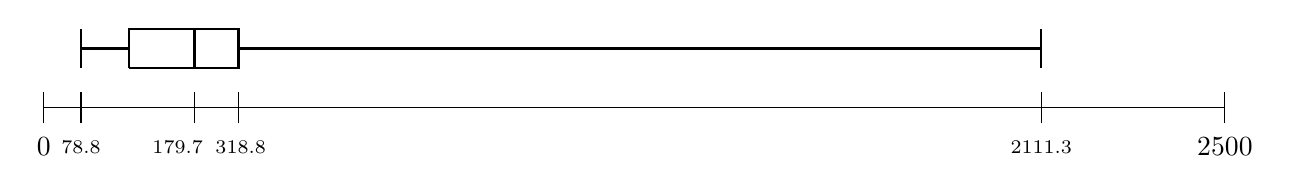
\begin{tikzpicture}
	\draw (0,0) -- (15,0);
	
	\draw[thick] (0.472,0.5) -- (0.472,1);
	\draw[thick] (0.472,0.75) -- (1.078,0.75);
	\draw[thick] (1.9128,0.5) -- (1.9128,1);
	\draw[thick] (1.078,0.5) -- (1.078,1) -- (2.472,1) -- (2.472,0.5) -- (1.078,0.5);
	\draw[thick] (2.472,0.75) -- (12.6675,0.75);
	\draw[thick] (12.6675,0.5) -- (12.6675,1);
	
	\draw (0,-0.2) -- (0,0.2); \node at (0, -0.5) {0};
	\draw (15,-0.2) -- (15,0.2); \node at (15, -0.5) {2500};
	\draw (0.472,-0.2) -- (0.472,0.2); \node at (0.472, -0.5) {\scriptsize 78.8};
	\draw (1.9128,-0.2) -- (1.9128,0.2); \node at (1.7, -0.5) {\scriptsize 179.7};
	\draw (2.472,-0.2) -- (2.472,0.2); \node at (2.5, -0.5) {\scriptsize 318.8};	
	\draw (12.6675,-0.2) -- (12.6675,0.2); \node at (12.6675, -0.5) {\scriptsize 2111.3};	
	\end{tikzpicture}
	\end{figure}
\end{enumerate}



\newpage



% Problem 2
\problem{10} Consider the following dataset:
	\[
	23, \qquad 38, \qquad 17, \qquad 20, \qquad 26
	\]

Showing all your work, complete the following: 
	\begin{enumerate}[(a)]
	\item Find the mean of for this dataset. 
	\item Find the standard deviation for this dataset. 
	\item If you increased each of the numbers above by 3, what happens to the mean and standard deviation? Explain. 
	\item Would the median or the mean be a more robust measure of center for this dataset? Explain. 
	\end{enumerate} \pspace

\sol 
\begin{enumerate}[(a)]
\item The mean of this dataset is\dots
	\[
	\overline{x}= \dfrac{\sum x_i}{n}= \dfrac{23 + 38 + 17 + 20 + 26}{5}= \dfrac{124}{5}= 24.8
	\]

\item Recall that the variance is $\sigma^2= \frac{1}{n - 1} \sum (x_i - \overline{x})^2$ and the standard deviation is $\sigma= \sqrt{\sigma^2}$. \par
	\begin{table}[h]
	\centering
	\begin{tabular}{ccc}
	$x_i$ & $x_i - \overline{x}$ & $(x_i - \overline{x})^2$ \\ \hline
	$23$ & $-1.8$ & $3.24$ \\
	$38$ & $13.2$ & $174.24$ \\
	$17$ & $-7.8$ & $60.84$ \\
	$20$ & $-4.8$ & $23.04$ \\
	$26$ & $1.2$ & $1.44$ \\ \hline
	& Total: & $262.8$
	\end{tabular}
	\end{table}
Therefore, the variance is\dots
	\[
	\sigma^2= \dfrac{1}{n - 1} \sum (x_i - \overline{x})^2= \dfrac{1}{5 - 1} \cdot 262.8= \dfrac{1}{4} \cdot 262.8= 65.7
	\]
But then the standard deviation is $\sigma= \sqrt{\sigma^2}= \sqrt{65.7}= 8.10555$. \pspace

\item Because each value would go up by 3, the mean would go up by 3. However, because all the values `stay in the same position' relative to all other numbers in the dataset, the total `spread' of the dataset must stay the same. Therefore, the standard deviation remains unchanged. Alternatively, if we introduce a linear change of variables $mx + b$, the mean changes from $\overline{x}$ to $m \overline{x} + b$ and the standard deviation is multiplied by a factor of $|m|$. \pspace

\item The median would be a more robust measure of center than the mean. The median is more resistant to the presence of outliers compared to the mean. If the value $10^{10}$ were added to the dataset, the mean would change to nearly $\frac{1}{5} \cdot 10^{10}$ whereas the median would merely change from 23 to 26. 
\end{enumerate}


\end{document}